\documentclass[a4paper,12pt]{report}
\usepackage[T2A]{fontenc}  %поддержка кириллицы в ЛаТеХ
\addtolength{\hoffset}{-1.7mm} % горизонтальное смещение всего текста как целого
\usepackage[utf8]{inputenc}  %По умолчанию кодировка KOI8 для *nix-систем
\usepackage[english,russian]{babel} %определение языков в документе
\usepackage{amssymb,amsmath,amsfonts,latexsym,mathtext} %расширенные наборы
  % математических символов
\usepackage{cite}  %"умные" библиографические ссылки
%(сортировка и сжатие)
\usepackage{indentfirst} %делать отступ в начале параграфа
\usepackage{enumerate}  %создание и автоматическая нумерация списков
\usepackage{tabularx}  %продвинутые таблицы
%\usepackage{showkeys}  %раскомментируйте, чтобы в документе были видны
%ссылки на литературу, рисунки и таблицы
\usepackage[labelsep=period]{caption} %заменить умолчальное разделение ':' на '.'
% в подписях к рисункам и таблицам
%\usepackage[onehalfspacing]{setspace} %"умное" расстояние между строк - установить
% 1.5 интервала от нормального, эквивалентно
 \renewcommand{\baselinestretch}{1.24}
\usepackage{graphicx} %разрешить включение PostScript-графики
\graphicspath{{Images/}} %относительный путь к каталогу с рисунками,это может быть мягкая ссылка

\usepackage{geometry} %способ ручной установки полей
\geometry{top=2cm} %поле сверху
\geometry{bottom=2.5cm} %поле снизу
\geometry{left=2.5cm} %поле справа
\geometry{right=2cm} %поле слева

\usepackage[colorlinks,linkcolor=blue]{hyperref}%гиперссылки в тексте
\newcommand{\tocsecindent}{\hspace{7mm}}% отступ для введения

\makeatletter
\bibliographystyle{unsrt} %Стиль библиографических ссылок БибТеХа - нумеровать
%в порядке упоминания в тексте
\renewcommand{\@biblabel}[1]{#1.}
\makeatother

\begin{document}
%Задаем определение
\newtheorem{Def}{Определение}

%Титулный лист
\begin{titlepage}
\newpage

\begin{center}
{\small\bfМИНИСТЕРСТВО ОБРАЗОВАНИЯ И НАУКИ РОССИЙСКОЙ ФЕДЕРАЦИИ\\
ОБНИНСКИЙ ИНСТИТУТ АТОМНОЙ ЭНЕРГЕТИКИ --- филиал}\\
федерального государственного автономного образовательного учреждения\\
высшего профессионального образования\\
{\bf<<Национальный исследовательский ядерный университет <<МИФИ>>\\
(ИАТЭ НИЯУ МИФИ)}\\
\vspace{2em}
Факультет кибернетики\\
Кафедра автоматизированных систем управления
\end{center}
\vspace{2em}
УДК 004.032.26
\hfill
\parbox{5.5cm}
{
ДОПУЩЕНА К ЗАЩИТЕ\\
Заведующий кафедрой АСУ\\
д.т.н., профессор\\
\hbox to 5.5cm{\dotfill А.Н. Анохин}
}
\vspace{5em}
\begin{center}
\textbf{ВЫПУСКНАЯ РАБОТА}
\end{center}

%\vspace{2em}

\begin{center}
АЛГОРИТМЫ ОБУЧЕНИЯ И АРХИТЕКТУРА НЕЙРОННЫХ СЕТЕЙ
\end{center}

\vspace{6em}

\hbox to \textwidth
{\parbox{6 cm}{Студент гр. ИНФ-Б08}\dotfill \parbox{4 cm}{
\begin{flushright}Белявцев~И.П.\end{flushright}}}
\vspace{2em}

\hbox to \textwidth
{\parbox{6 cm}{Руководитель\\ заведующий кафедрой КССТ\\ д.т.н.}\dotfill \parbox{4 cm}{
\begin{flushright}Старков~С.О.\end{flushright}}}
\vspace{2em}

\hbox to \textwidth
{\parbox{6 cm}{Рецензент\\ научный сотрудник О-ЦОД, \\
ФГБУ <<ВНИИГМИ-МЦД>>\\к.т.н.}\dotfill \parbox{4 cm}{
\begin{flushright}Белов~С.В.\end{flushright}}}

\vspace{\fill}

\begin{center}
Обнинск 2012
\end{center}

\end{titlepage}
\setcounter{page}{2} % начать нумерацию с номера три

%Реферат
\begin{center}
\section*{Реферат}
\end{center}

\vspace{2em}
41 стр., 15 рис., 3 ист.

\vspace{2em}
РАСПОЗНАВАНИЕ ИЗОБРАЖЕНИЙ, ИСКУССТВЕННАЯ НЕЙРОННАЯ СЕТЬ, ТОПОЛОГИИ, АЛГОРИТМЫ ОБУЧЕНИЯ, ПАРАДИГМЫ ОБУЧЕНИЯ, ОБЪЕКТНО-ОРИЕНТИРОВАННОЕ ПРОГРАММИРОВАНИЕ, {\it UML}, {\it JAVA}

\vspace{2em}
Объектом исследования являются алгоритмы обучения и топологии искусственных нейронных сетей.

Цель работы --- программная реализация искусственной нейронной сети в объектно-ориентированной парадигме программирования.

В данной работе исследуются математические модели нейронов, топологии нейронных сетей, алгоритмы и парадигмы обучения нейронных сетей.
Проводится работа по созданию однослойной нейронной сети прямого распространения для распознавания образов арабских цифр.
Искусственная нейронная сеть создается в объектно-ориентированной парадигме программирования и на языке программирования {\it Java}.

Полученная искусственная нейронная сеть используется для исследования влияния количества циклов обучения, параметра скорости обучения и коэффициента наклона сигмоидальной функции на качество обучения и качество последующей работы нейронной сети.

%Меняем название Оглавления
\renewcommand{\contentsname}{\begin{center}Содержание\end{center}}
%Оглавление
\tableofcontents 
\newpage

%Список сокращений
\begin{center}
\section*{Обозначения и сокращения}
\end{center}

ИНС --- искусственная нейронная сеть.

БНС --- биологическая нейронная сеть.

ЭВМ --- электронно-вычислительная машина.


\newpage

%Введение
\begin{center}
\section*{Введение}
\addcontentsline{toc}{section}{\tocsecindent{Введение}}
\end{center}


Длительный период биологической эволюции придал мозгу человека много качеств, которые отсутствуют как в машинах с архитектурой фон Неймана, так и в современных параллельных компьютерах.
К ним относятся:
\begin{itemize}
\item[-] массовый параллелизм
\item[-] распределенное представление информации и вычисления
\item[-] способность к обучению
\item[-] способность к обобщению
\item[-] адаптивность
\item[-] свойство контекстуальной обработки информации
\item[-] толерантность к ошибкам
\item[-] низкое энергопотребление
\end{itemize}
Можно предположить, что приборы и системы, построенные на тех же принципах, что и биологические нейроны, будут наследовать эти свойства.

Существует множество подходов к реализации искусственной нейронной сети (ИНС).
При этом большинство реализации основаны на функциональной парадигмы программирования (язык программирования {\it Lisp}).
При этом существует очень мало реализаций ИНС в объектно-ориентированной парадигме программирования.

Поэтому целью данной работы является реализация искусственной нейронной сети на языке {\it Java} для распознавания образов арабских цифр, представленных монохромными изображениями.
Для достижения поставленной цели необходимо выполнить следующие шаги:
\begin{enumerate}
\item изучить теоретические основы моделирования нейронных сетей;
\item реализовать ИНС на языке {\it Java} для распознавания арабских цифр;
\item исследовать влияние параметров нейронной сети на процесс распознавания символов.
\end{enumerate}


\newpage

%Основная часть
%\chapter{Исследование предметной области}
	%Обшее определение искусственных нейронных сетей
	\chapter{Искусственные нейронные сети}
\section{Общее определение искусственной нейронной сети}

Искусственными нейронными сетями (ИНС) называется совокупность моделей биологических нейронных сетей.
ИНС представляет собой сеть искусственных нейронов, связанных между собой искусственными синаптическими соединениями.
Сеть обрабатывает входную информацию и в процессе изменения своего состояния во времени формирует совокупность выходных сигналов.\cite{COURSE}
Так как ИНС моделирует реальную нейронную сеть, рассмотрим принципы функционирования биологического образца.
Структурной единицей биологической нейронной сети является нейрон (нервная клетка).
\begin{figure}[h]
\center{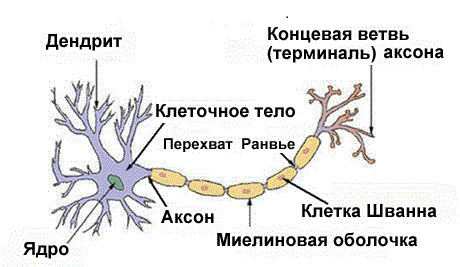
\includegraphics{Neuron.png}}
\caption{Структура нейрона}
\label{ris:neuron}
\end{figure}
Нейрон (рис.~\ref{ris:neuron}) является особой биологической клеткой, корорая обрабатывает информацию.
Она состоит из тела клетки, или сомы, и двух внешних древоподобных ветвей: аксона и дендритов.
Тело клетки включает ядро, которое содержит информацию о наследственных свойствах, и плазму, обладающую молекулярными средствами для производства необходимых нейрону материалов.
Нейрон получает сигналы (импульсы) от других нейронов через дендриты и передают сигналы, сгенерированные телом клетки, вдоль аксона, который в конце разветвляется на волокна.
На окончаниях этих волокон находятся синапсы. 
Синапс является элементарной структурой и функциональным узлом между двумя нейронами (волокно аксона одного нейрона и дендрит другого).
Когда импульс достигает синаптического окончания, высвобождаются определенные химические вещества, называемые нейротрансмиттерами.
Нейротрансмиттеры диффундируют через синаптическую щель, возбуждая или затормаживая, в зависимости от типа синапса, способность нейрона-приемника генерировать электрические импульсы.
Результативность синапса может настраиваться проходящими через него сигналами, так что синапсы могут обучаться в зависимости от активности процессов, в которых они участвуют.
Эта зависимость от предыстории действует как память, которая, возможно, ответственна за память человека.
\cite{nn_int_jain}
Созданные из таких структурных элементов биологический нейронные сети обладают следующими свойствами:
\begin{itemize}
\item[-] {\bfПараллельность обработки информации. }
Каждый нейрон формирует свой выход только на основе своих входов и собственного внутреннего состояния под воздействием общих механизмов регуляции нервной системы.
\item[-] {\bfСпособность к полной обработке информации. }
Все известные человеку задачи решаются нейронными сетями.
К этой группе свойств относятся ассоциативность (сеть может восстанавливать полный образ по его части), способность к классификации, обобщению, абстрагированию и множество других.
\item[-] {\bfСамоорганизация.}
В процессе работы БНС самостоятельно, под воздействием внешней среды, обучаются решению разнообразных задач.
Неизвестно никаких принципиальных ограничений на сложность задач, решаемых БНС.
Нервная система сама формирует алгоритмы своей деятельности, уточняя и усложняя их в течении жизни.
\item[-] {\bfНаждежность. }
Биологические НС обладают фантастической надежностью: выход из строя даже 10\% нейронов в нервной системе не прерывает ее работы. 
По сравнению с последовательными ЭВМ, основанными на принципах фон-Неймана, где сбой одной ячейки памяти или одного узла в аппаратуре приводит к краху системы.\cite{COURSE}
\end{itemize}


	%Математические модели работы нейронов
	\section{Математические модели работы нейронов}
\subsection{Детерминистская модель}
\begin{figure}[h]
\center{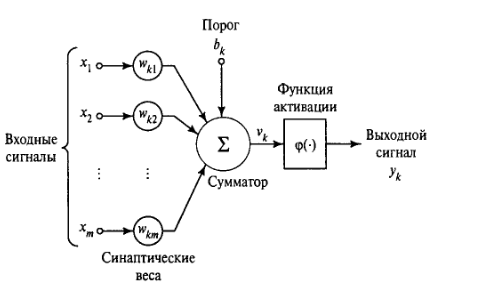
\includegraphics[width=0.8\linewidth]{BlockSheme.png}}
\caption{Явная нелинейная модель нейрона.}
\label{ris:BlockScheme}
\end{figure}
Как было выяснено ранее, нейрон представляет собой единицу обработки информации в нейронной сети. 
На блок-схеме рис.~\ref{ris:BlockScheme} показана модель нейрона, лежащая в основе искусственных нейронных сетей.
В этой модели можно выделить три основных функциональных элемента.
\begin{enumerate}
\item Набор синапсов или связей, каждый из которых характеризуется своим весом или силой.
В частности, сигнал $x_j$ на входе синапса $j$, связанного с нейроном $k$, умножается на вес $\omega_{jk}$.
В отличии от синапсов мозга синаптический вес искусственного может принимать как положительные, так и отрицательные значения. 
\item Сумматор складывает входные сигналы, взвешенные относительно соответствующих весов синапсов нейронов.
Математически эту операцию можно описать как линейную комбинацию входных сигналов.
\item Функция активации ограничивает выходную амплитуду сигнала нейрона.
Эта функция также называется функцией сжатия.
Обычно выходной сигнал нормализуется в диапазоне $[0;1]$ или $[-1;1]$.
\end{enumerate}
В модель нейрона, показанную на рис.~\ref{ris:BlockScheme}, включён пороговый элемент, который обозначается символом $b_k$.
Эта величина отражает увеличение или уменьшение входного сигнала функции активации.
В математической форме функционирование нейрона $k$ можно описать следующей парой уравнений:
\begin{equation}
u_k = \sum_{j=1}^{m} \omega_{kj}x_j
\end{equation}
\begin{equation}
y_k = \varphi (u_k + b_k)
\end{equation}
где $x_1,x_2,\dots,x_m$ --- входные сигналы;
$\omega_{k1},\omega_{k2},\dots,\omega_{km}$ --- синаптические веса нейрона $k$;
$u_k$ --- линейная комбинация входных воздействий;
$b_k$ --- порог;
$\varphi()$ --- функция активации;
$y_k$ --- выходной сигнал нейрона.\cite{NejronnyeSeti}
\subsection{Функции активации}
Функция активации, представленные в формулах как $\varphi()$, определяет выходной сигнал нейрона.
Можно выделить три основных типов функции активации.
\begin{enumerate}
\item Функция единичного скачка, или пороговая функция.
Этот тип функции описывается следующим уравнением:
\begin{equation}
\varphi(v) = 
\begin{cases}
1, v \ge 0\\
0, v < 0
\end{cases}
\end{equation}
В технической литературе эта форма функции единичного скачка называется функцией Хэвисайда.
Соответственно выходной сигнал нейрона $k$ можно представить как
\begin{equation}
y_k = 
\begin{cases}
1, v_k \ge 0\\
0, v_k < 0
\end{cases}
\end{equation}
где $v_k$ --- индуцированное локальное поле нейрона $k$.
Эту модель в литературе называют моделью Мак-Каллока-Питца. В этой модели выходной сигнал нейрона принимает значение 1 при неотрицательном индуцированном локальным полем, и 0 --- в противном случае.
Это выражение описывает свойство <<все или ничего>> модели Мак-Каллока-Питца.
\item Кусочно-линейная функция. Кусочно-линейная функция описывается следующим выражений:
\begin{equation}
\varphi(v) = 
\begin{cases}
1, v \ge +\frac12\\
|v|, -\frac12<v<+\frac12\\
0, v \le -\frac12
\end{cases}
\end{equation}
где коэффициент усиления в линейной области оператора предполагается равным единице.
Следующие два варианта можно считать особой формой кусочно-линейной функции.
\begin{itemize}
\item Если линейная область не достигает порога насыщения, они превращается в линейный сумматор 
\item Если коэффициент усиления линейной области стремиться к бесконечности, то кусочно-линейная функция выражается в пороговую.
\end{itemize}
\item Сигмоидальная функция. 
Сигмоидальная функция, график которой напоминает букву S, является наиболее распространённой функцией для построения искусственных нейронных сетей.
Это быстрорастущая функция, поддерживающая баланс между линейным и нелинейным поведением.
Примером сигмоидальной функции может служить логистическая функция, задаваемая выражением:
\begin{equation}
\varphi(v) = \frac1{1+e^{-av}}
\end{equation}
где $a$ --- параметр наклона сигмоидальной функции.
Изменяя этот параметр можно построить функции с различной крутизной.
При бесконечно большом параметре наклона функция вырождается в пороговую.
Если пороговая функция принимает только два значения (0 и 1), то сигмоидальная функция принимает бесконечное количество значений в диапазоне $[0;1]$.
При этом сигмоидальная функция является в отличии от пороговой дифференцируемая.\cite{NejronnyeSeti}
\end{enumerate}
\subsection{Стохастическая модель}
Модель нейрона, рассмотренная выше, является строго детерминистской.
Это значит, что преобразование входного сигнала в выходной точно определено для всех значений входного сигнала.
Однако в некоторых случаях предпочтительно использовать стохастические (вероятностные) нейросетевые модели.
В подобных моделях нейрон находится в одном из двух состояний (+1 и -1).
Решение о переключении нейрона из одного состояния в другое производится с учётом вероятности этого события.
Обозначим состояние нейрона символом $x$, а вероятность активации нейрона --- функцией $P(v)$, где $v$ --- локальное индуцированное поле нейрона.
Тогда
\begin{equation}
x=
\begin{cases}
+1, \text{с вероятностью } P(v),\\
-1, \text{с вероятностью } 1-P(v)
\end{cases}
\end{equation}
Вероятность $P(v)$ описывается сигмоидальной функцией следующего вида:
\begin{equation}
P(v) = \frac1{1 + e^{- v/T}}
\end{equation}
где $T$ --- это аналог температуры, используемый для управления уровнем шума, и таким образом, степенью неопределённости переключения.
При этом параметр $T$ не имеет отношения к физической температуре. \cite{NejronnyeSeti}

	%Топологии нейронных сетей
	\subsection{Топологии нейронных сетей}

Структура нейронных сетей тесно связана с используемыми алгоритмами обучения.
В общем случае можно выделить три фундаментальных архитектуры нейронных сетей.

\subsubsection{Однослойные прямого распространения}

В многослойных нейронной сети нейроны располагаются по слоям.
В простейшем случае у такой сети существует входной слой узлов источника, информация от которого передается на выходной слой нейронов (вычислительные узлы), но не наоборот. 
Такая сеть называется сетью прямого распространения или ациклической сетью.
\begin{figure}[h]
\center{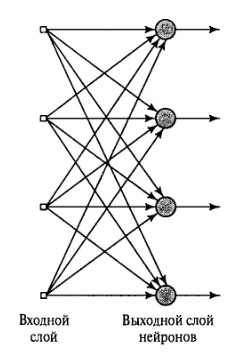
\includegraphics[width=0.4\linewidth]{OneLayer.png}}
\caption{Однослойная сеть прямого распространения}
\label{ris:OneLayer}
\end{figure}

На рис.~\ref{ris:OneLayer} показана структура такой сети для случая четырёх узлов в каждом из слоев (входном и выходном).
Такая нейронная сеть называется однослойной, при этом под единственным слоем подразумевается слой вычислительных элементов (нейронов).
При подсчёте числа слоев мы не принимаем во внимание узлы источника, так как они не выполняют никаких вычислений.\cite{NejronnyeSeti}

\subsubsection{Многослойные прямого распространения}

Другой класс нейронных сетей прямого распространения  характеризуется наличием одного или нескольких скрытых слоев, узлы которых называют скрытыми нейронами или скрытыми элементами.
Функция последних заключается в посредничестве между внешним входным сигналом и выходом нейронной сети.
Добавляя один или несколько нейронных слоев мы можем выделить статистики более высокого порядка.
Такая сеть позволяет выделять глобальные свойства данных с помощью локальных соединений за счёт наличия дополнительных синаптических связей  и повышения уровня взаимодействий нейронов.
Способность скрытых нейронов выделять статистические зависимости высокого порядка особенно существенна, когда размер входного слоя достаточно велик.

Узлы источника входного слоя сети формируют соответствующие элементы шаблона активации (входной  вектор), которые составляют входной сигнал, поступающий на нейроны (вычислительные элементы) второго слоя (т.е. первого скрытого слоя).
Выходные сигналы второго слоя используются в качестве входных для третьего слоя и т.д.
Обычно нейроны каждого из слоев сети используют в качестве входных сигналов только выходные сигналы нейронов предыдущего слоя.
Набор выходных сигналов нейронов последнего слоя сети определяет общий отклик сети на данный входной образ, сформированный узлами источника входного слоя.

\begin{figure}[h]
\center{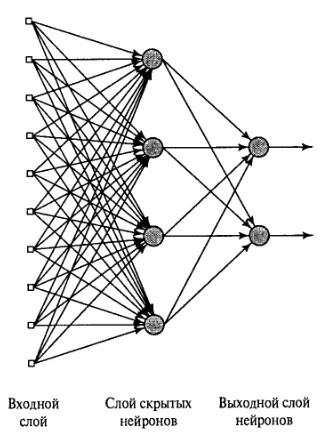
\includegraphics[width=0.4\linewidth]{ManyLayer.png}}
\caption{Многослойная сеть прямого распространения}
\label{ris:ManyLayer}
\end{figure}

Сеть, показанная на рис.~\ref{ris:ManyLayer}, называется сетью 10-4-2, так как имеет 10 входных, 4 скрытых и 2 выходных нейрона.
Нейронная сеть, показанная на рис.~\ref{ris:ManyLayer}, считается полносвязной в том смысле, что все узлы каждого конкретного слоя соединены со всеми узлами смежных слоев.
Если некоторые из синаптических связей отсутствуют, то такая сеть называется неполносвязной.\cite{NejronnyeSeti}

\subsubsection{Рекуррентные}
Рекуррентная нейронная сеть отличается от сетей прямого распространения наличием по крайней мере одной обратной связи.
Например, рекуррентная сеть может состоять из единственного слоя нейронов, каждый из которых направляет выходной сигнал на входы всех остальных нейронов сети.

\begin{figure}[h]
\center{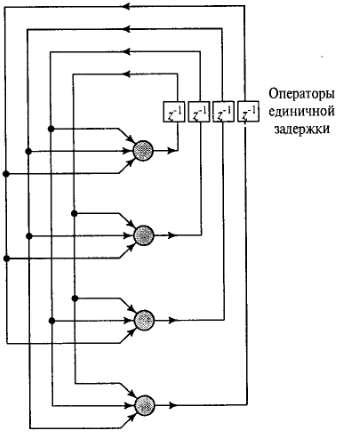
\includegraphics[width=0.4\linewidth]{Recurrent.png}}
\caption{Рекуррентная сеть без скрытых нейронных слоев}
\label{ris:Recurrent}
\end{figure}

Архитектура нейронной сети показана на рис.~\ref{ris:Recurrent}.
Стоит обратить внимание, что в нейронной сети нет обратной связи нейронов самих с собой.
Рекуррентная сеть, показанная на рис.~\ref{ris:Recurrent}, не имеет скрытых нейронов.
Наличие обратных связей в нейронных сетях оказывает непосредственное влияние на способность таких сетей к обучению и на их производительность.
Более того, обратная связь подразумевает наличие элементов единичной задержки, что приводит к нелинейному динамическому поведению.\cite{NejronnyeSeti}
	%Модели обучения нейронных сетей
	\section{Алгоритмы обучения нейронных сетей}

Самым важным свойством нейронных сетей является их способность обучаться на основе данных окружающей среды и в  результате обучения повышать свою производительность.
Повышение производительности происходит со временем в соответствии с определёнными правилами.
Обучение нейронной сети происходит посредством интерактивного
процесса корректировки синаптических весов и порогов.
В идеальном случае нейронная сеть получает знания об окружающей среде на каждой итерации процесса обучения.

С понятием обучения ассоциируется довольно много видов деятельности, поэтому сложно дать этому процессу однозначное определение.
С позиций нейронных сетей мы можем использовать следующее определение обучения
Обучение ---  это процесс, в котором свободные параметры нейронной сети настраиваются посредством моделирования среды, в которую эта сеть встроена.
Тип обучения определяется способом подстройки этих параметров. 

Это определение предполагает следующую последовательность событий при обучении нейронной сети:

\begin{enumerate}
	\item В нейронную сеть поступают стимулы из внешней среды.

	\item В результате этого изменяются свободные параметры нейронной сети.

	\item После изменения внутренней структуры нейронная сеть отвечает на возбуждения уже иным образом.
\end{enumerate}

Вышеуказанный список четких правил решения проблемы обучения называется алгоритмом обучения. 
Несложно догадаться, что не существует универсального алгоритма обучения, подходящего для всех архитектур нейронных сетей.
Существует лишь набор средств, предоставленный множеством алгоритмов обучения, каждый из которых имеет свои достоинства.\cite{NejronnyeSeti}

\subsection{Обучение на основе коррекции ошибок}

Для того, чтобы проиллюстрировать первое правило обучения, рассмотрим простейший случай нейрона $k$ --- единственного вычислительного узла выходного слоя нейронной сети прямого распространения.
Нейрон $k$ работает под управлением вектора сигнала $\vec x (n)$, производимого одним или несколькими скрытыми слоями нейронов, которые в свою очередь получают информацию из входного вектора, передаваемого начальным узлам нейронной сети.
Под $n$ подразумевается дискретное время или, более конкретно, --- номер шага итеративного процесса настройки синаптических весов нейрона $k$.
Выходной сигнал нейрона $k$ обозначается $y_k(n)$.
Этот сигнал будет сравниваться с желаемым выходом, обозначенным $d_k(n)$.
В результате получим сигнал ошибки $e_k(n)$.
По определению
\begin{equation}
e_k(n) = y_k(n) - d_k(n)
\end{equation}

Сигнал ошибки инициализирует механизм управления, цель которого заключается применении последовательности корректировок к синаптическим весам нейрона $k$.
Эти изменения нацелены на пошаговое приближение выходного сигнала $y_k(n)$ к желаемому $d_k(n)$.
Эта цель достигается за счет минимизации функции стоимости или индекса производительности $E(n)$, определяемой в терминах сигнала ошибки следующим образом:
\begin{equation}
E(n) = \frac12 e_k^2(n)
\end{equation}
где $E(n)$ --- текущее значение энергии ошибки.
Пошаговая корректировка синаптических весов нейрона $k$  продолжается пока до тех пор, пока система не достигнет устойчивого состояния.
В этой точке процесс обучения останавливается.

Процесс, описанный выше, называется обучением на основе коррекции ошибок.
Минимизация функции стоимости $E(n)$ выполняется по так называемому дельта-правилу, или правилу Видроу-Хоффа, названному в честь его создателей.
Обозначим $\omega_{kj}(n)$  текущее значение синаптического веса $\omega_{kj}$ нейрона $k$, соответствующему элементу $x_j(n)$ вектора $\vec x(n)$, на шаге дискретизации $n$.
В соответствии с дельта-правилом изменение $\Delta\omega_{kj}(n)$, применяемое  к синаптическому весу $\omega_{kj}$ на этом шаге дискретизации, задается выражением
\begin{equation}
\Delta\omega_{kj}(n) = \eta e_k(n)x_j(n)
\end{equation}
где $\eta$ --- некоторая положительная константа, определяющая скорость обучения и используемая при переходе  от одного шага процесса к другому. 
Эту константу естественно именовать параметром скорости обучения.
Вербально дельта-правило можно определить следующим образом:

Корректировка, применяемая к синаптическому весу нейрона, пропорциональна произведению сигнала ошибки на входной сигнал, его вызвавший.

Необходимо помнить, что  определенное таким образом дельта-правило предполагает возможность прямого измерения сигнала ошибки.
Для обеспечения такого измерения требуется поступление желаемого отклика от некоторого внешнего источника, непосредственно доступного для нейрона $k$.
Другими словами нейрон $k$ должен быть видимым для внешнего мира.
Вычислив величину изменения синаптического веса $\Delta\omega_{kj}(n)$, можно определить его новое значение для следующего шага дискретизации:
\begin{equation}
\Delta\omega_{kj}(n+1) = \omega_{kj}(n) +\Delta\omega_{kj}(n)
\end{equation}

\subsection{Конкурентное обучение}

Как следует из самого названия, в конкурентном обучении выходные нейроны нейронной сети конкурируют между собой за право быть активизированными.
Благодаря этому свойству конкурентное обучение очень удобно использовать для изучения статистических свойств, используемых в задачах классификации входных образов. 
Правило конкурентного обучения основано на использовании трех основных элементов.
\begin{itemize}
\item Множество одинаковых нейронов со случайно распределенными синаптическими весами, приводящими к различной реакции нейронов на один и тот же входной сигнал.
\item Предельное значение <<силы>> каждого нейрона
\item Механизм, позволяющий нейронам конкурировать за право отклика на данное подмножество входных сигналов  и определяющий единственный активный выходной нейрон.
Нейрон, победивший в этом соревновании, называют нейроном-победителем, а принцип конкурентного обучения формулируют в виде лозунга <<победитель забирает все>> 
\end{itemize}

	%Парадигмы обучения нейронных сетей
	\section{Парадигмы обучения нейронных сетей}

\subsection{Обучение с учителем}

Рассмотрим парадигмы обучения нейронных сетей.
Начнем с парадигмы обучения с учителем.

\begin{figure}[h]
\center{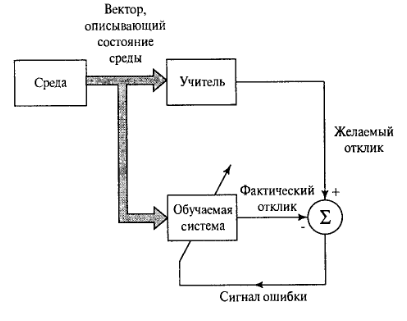
\includegraphics[width=0.6\linewidth]{WithTeacher.png}}
\caption{Блочная диаграмма обучения с учителем.}
\label{ris:WithTeacher}
\end{figure}

На рис.~\ref{ris:WithTeacher} приведена блочная диаграмма, иллюстрирующая эту форму обучения. 
Концептуально участие учителя можно рассматривать как наличие знаний об окружающей среде, представленных в виде пар вход-выход.
При этом сама среда неизвестна обучаемой нейронной сети.
Теперь предположим, что учителю и обучаемой сети подается  из окружающей среды вектор.
На основе встроенных знаний учитель может сформировать и передать обучаемой нейронной сети желаемый отклик, соотвествующий входному вектору.
Этот желаемый результат представляет оптимальные дествия, которые должна выполнить нейронная сеть.
Параметры сети корректируются с учетом обучающего вектора и сигнала ошибки.
Корректировка параметров должна выполняться пошагово с целью иммитации нейронной сетью поведения учителя.
Эта эмуляция в некотором статистическом смысле должна быть оптимальной.
Таким образом, в процессе обучения знания учителя передаются в сеть в максимально полном объеме.
 

\subsection{Обучение без учителя}

Обучение без учителя осуществляется без вмешательства внешнего учителя или корректора, контроллирующего процесс обучения.
Существует лишь независимаю мера качества представления, которому должна научиться нейронная сеть, и свободные парамтеры сети оптимизируются по отношению к этой мере.
После обучения сети на статистические закономерности входного сигнала она способна формировать внутреннее представление кодируемых признаков входных данных, и таким образом, автоматически создавать новые классы.

Для обучения без учителя можно воспользоваться правилом конкурентного обучения.
Например, можно использовать нейронную сеть, состоющую из двух слоев --- входного и выходного.
Входной слой получает доступные данные.
Выходной слой состоит из нейронов, конкурирующих друг с другом за право отклика на признаки, содержащиеся во входных данных.
В простейшем случае нейронная сеть действет по принципу <<победтель забирает всё>>.
При этом все остальные нейроны отключаются.

%\chapter{Практическая реализация искусственной нейронной сети}	
	%Постановка задачи распознавания 
	\section{Практическая реализация искусственной нейронной сети}	
\subsection{Постановка задачи}

В качестве практической иллюстрации положений из теоретической части необходимо программно реализовать ИНС.
Для реализации искусственной нейронной сети необходимо воспользоваться объектно-ориентированным подходом и реализовать программу на языке {\it Java}.
Нейронная сеть на вход должна получать монохромное изображение арабской цифры размером 64 на 64 пиксела в формате {\it JPG}.
На выходе нейронной сети должна быть вероятность того, что на изображении присуствует та или иная цифра.

С точки зрения топологии нейронных сетей реализуемая нейронная сеть представляет собой однослойную сеть прямого распространения с 4096 входными нейронами и 10 выходными нейронами.
В качестве алгоритма обучения необходимо воспользоваться алгоритмом обратного распространения ошибки.

Должен быть реализован режим проверки работоспособности и режим обучения.
В режиме проверки работоспособности на вход нейронной сети подается файл с изображением, а на выходе должна быть рассчитана вероятность того, что в файле изображена какая-либо цифра
В режиме обучения сеть проходит заданое количество циклов обучения с определенными параметрами скорости обучения $\eta$ и параметром наклона сигмоидальной функции $a$.
По заврешении обучения строится график завимости корректируемой ошибки от количества итераций обучения.


	%UML проектирование
	\subsection{UML-проектирование}

Первоначальной стадией разработки программного продукта является стадия проектирования.
В качестве проектного {\it CASE}-средства был выдран продукт {\it Visual Paradigm}.
С помощью его было составлена диаграмма классов (см. рис. ~\ref{ris:UML}), на основе которой был сгенерирован начальный код программного решения.

\begin{figure}[h]
\center{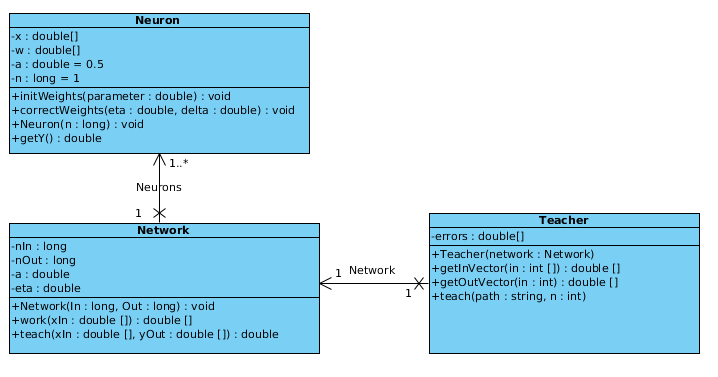
\includegraphics[width=1\linewidth]{uml}}
\caption{Диаграмма классов программного решения}
\label{ris:UML}
\end{figure}
	
	%Обучение и результат работы программы
	\subsection{Результат работы программы}


В режиме проверки до обучения ИНС демонстрирует абсолютную неспособность распознаванию образов (см. рис.~\ref{ris:Check}).

\begin{figure}[h]
\center{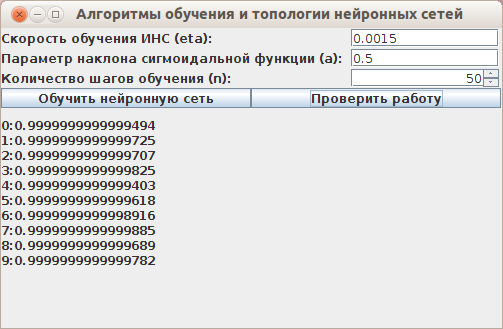
\includegraphics[width=0.75\linewidth]{check.png}}
\caption{Режим проверки до обучения}
\label{ris:Check}
\end{figure}

Обучим нейронную сеть с различными параметрами обучения.
Проведем 50 циклов обучения сети с параметрами скорости обучения 0,0015, 0,15 и 15 (см. рис.~\ref{ris:stud_0,0015_0,5_50}, \ref{ris:stud_0,15_0,5_50} и \ref{ris:stud_15_0,5_50}).

\begin{figure}[H]
\center{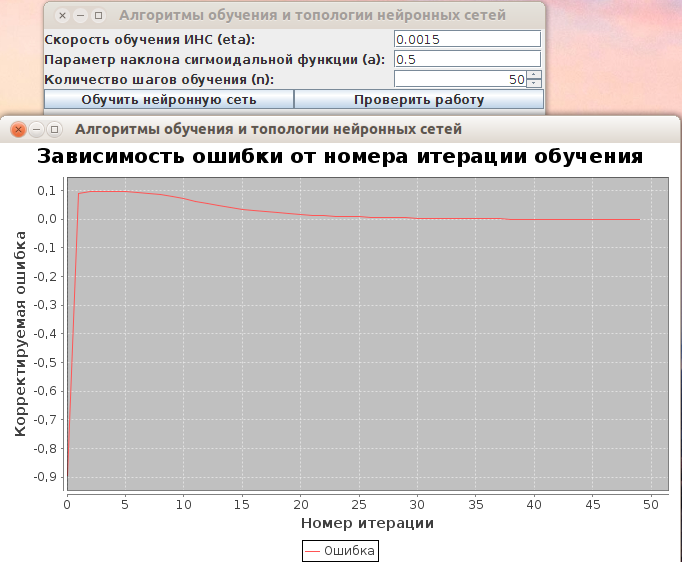
\includegraphics[width=0.75\linewidth]{stud_0,0015_0,5_50.png}}
\caption{Режим обучения. (Скорость обучения 0,0015. Параметр сигмоидальной функции 0,5. 50 циклов обучения)}
\label{ris:stud_0,0015_0,5_50}
\end{figure}

\begin{figure}[H]
\center{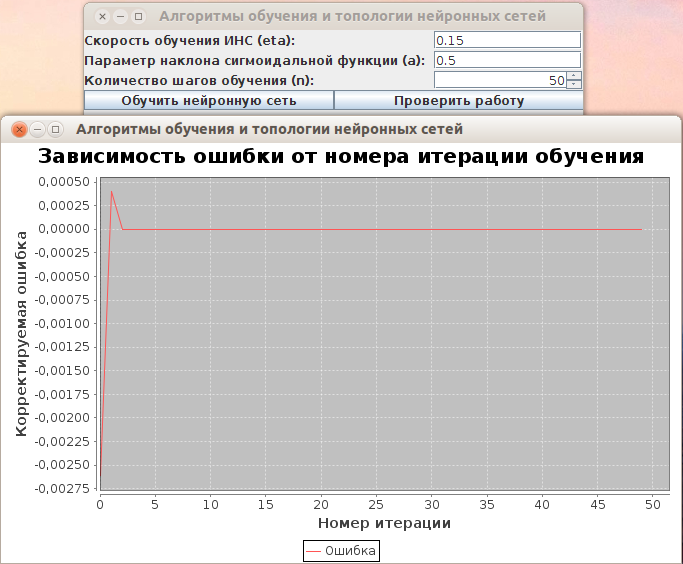
\includegraphics[width=0.75\linewidth]{stud_0,15_0,5_50.png}}
\caption{Режим обучения. (Скорость обучения 0,15. Параметр сигмоидальной функции 0,5. 50 циклов обучения)}
\label{ris:stud_0,15_0,5_50}
\end{figure}

\begin{figure}[H]
\center{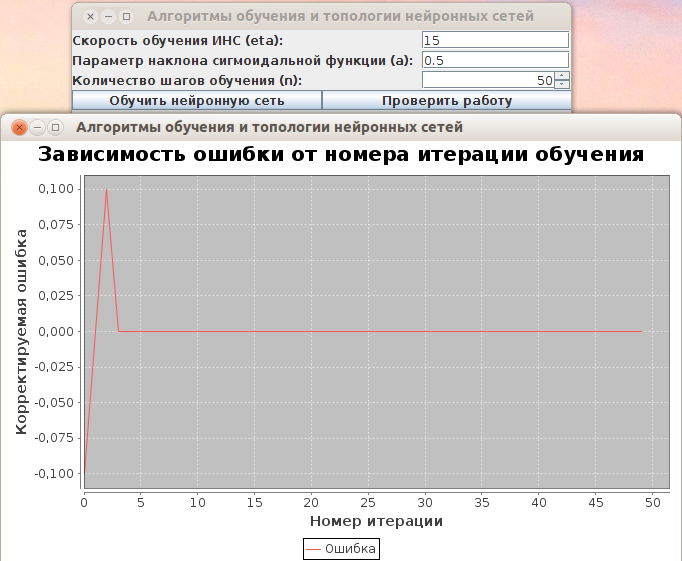
\includegraphics[width=0.75\linewidth]{stud_15_0,5_50.png}}
\caption{Режим обучения. (Скорость обучения 15. Параметр сигмоидальной функции 0,5. 50 циклов обучения)}
\label{ris:stud_15_0,5_50}
\end{figure}

Согласно полученным результатам коэффициент скорости обучения пропорционально влияет на скорость обучения. 
Однако при больших значениях возникает вероятность переобучения сети, т.е. увеличение ошибки от итерации к итерации.


Проведем 100 циклов обучения сети с параметром скорости обучения 0,0015 (см. рис.~\ref{ris:stud_0,0015_0,5_100}).

\begin{figure}[h]
\center{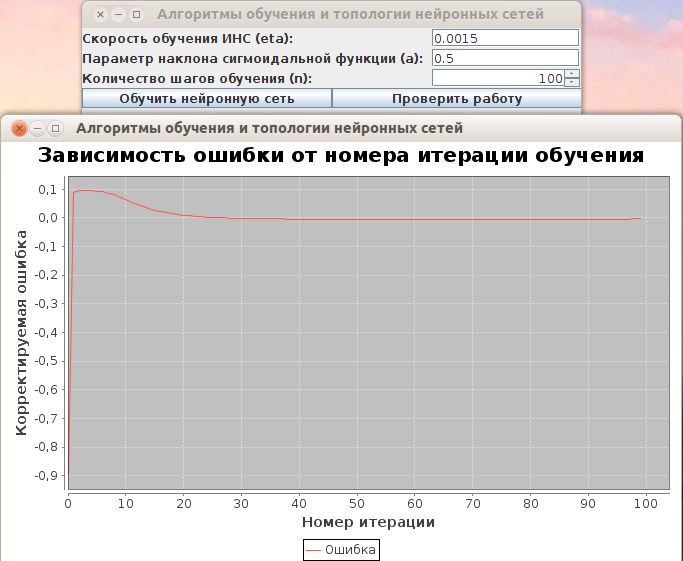
\includegraphics[width=0.75\linewidth]{stud_0,0015_0,5_100.png}}
\caption{Режим обучения. (Скорость обучения 0,0015. Параметр сигмоидальной функции 0,5. 100 циклов обучения)}
\label{ris:stud_0,0015_0,5_100}
\end{figure}

Согласно этим результатам ошибка нейронной сети уменьшается с каждой итерацией обучения.

Проведем 50 циклов обучения сети с параметром скорости обучения 0,0015 и коэффициентами наклона сигмоидальной функции 0,5 и 2,0, а затем проверим работу сети (рис.~\ref{ris:check_0,0015_0,5_50} и \ref{ris:check_0,0015_2,0_50}).

\begin{figure}[h]
\center{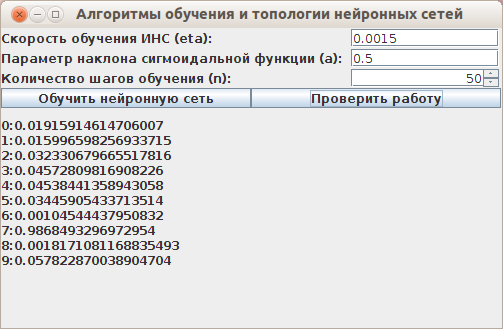
\includegraphics[width=0.75\linewidth]{check_0,0015_0,5_50.png}}
\caption{Режим проверки. (Скорость обучения 0,0015. Параметр сигмоидальной функции 0,5. 50 циклов обучения)}
\label{ris:check_0,0015_0,5_50}
\end{figure}

\begin{figure}[h]
\center{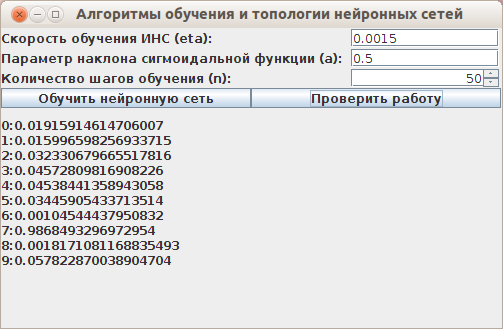
\includegraphics[width=0.75\linewidth]{check_0,0015_0,5_50.png}}
\caption{Режим проверки. (Скорость обучения 0,0015. Параметр сигмоидальной функции 2,0. 50 циклов обучения)}
\label{ris:check_0,0015_2,0_50}
\end{figure}

По результатам проверки видно, что коэффициент наклона сигмоидальной функции влияет на допустимые погрешности работы сети. Чем меньше этот коэффициент, тем сильнее сигмоидальная функция стремиться к пороговой.
%Заключение
\begin{center}
\section*{Заключение}
\addcontentsline{toc}{section}{\tocsecindent{Заключение}}
\end{center}

В данной выпускной работе были детально рассмотрены основы создания программных моделей нейронных сетей.
Были рассмотрены общие принципы моделирования, топологии, методы и парадигмы обучения.

В ходе практической реализации была создана объектно-ориентированная модель нейронной сети на языке {\it Java}.
Был реализован алгоритм обратного распространения ошибки для решения задачи распознавания образов арабских цифр.
Было выяснено, что однослойная сеть прямого распространения способна должным образом определять образы цифр из монохромных изображений малого разрешения (64 на 64 пикселя).

Опятным путем было показано влияние параметра скорости обучения на необходимое для правильной работы число циклов обучения.
Также опытным путем было выяснено, что сигнал ошибки нейронной сети немонотонно убывает с ростом числа циклов обучения.
Было показано, что коэффициент сигмоидальной функции влияет на ее наклон, а, следовательно, на толерантность работы сети.

Таким образом, на практике были подтверждены следующие свойства искуственных нейронных сетей:
\begin{itemize}
\item[-] Способность к обучению --- нейронная сеть после обучения способна определять образ цифры;
\item[-] Толерантность к ошибкам --- регулируется коэффициентом наклона сигмоидальной функции.
\end{itemize}


\newpage
%Список литературы
%\renewcommand{\bibname}{\begin{center}Список использованных источников\end{center}}
\renewcommand\refname{\centering Список использованных источников}
\addcontentsline{toc}{section}{\tocsecindent{Список использованных источников}}

\begin{thebibliography}{99}
\bibitem{NejronnyeSeti}
Хайкин~С. Нейронные сети: полный курс, 2-е издание : Пер. с англ. --- 
М.: Издательский дом <<Вильямс>>, 2006. --- 1104 с.: ил.
\bibitem{COURSE}
Заенцев~И.В. Нейронные сети: основные модели --- 
Воронеж: <<Воронеж>>, 1999. --- 76 с.: ил.
\bibitem{nn_int_jain}
Джейн А., Мао Ж. Введение в искусственные нейронные сети. --- 
Препринт статьи, 1996 ---  16 с.: ил.
\end{thebibliography}
%Исходники
	\section*{Приложение А. Исходный код программы}
\addcontentsline{toc}{section}{\tocsecindent{Приложение 1. Исходный код программы}}

\begin{verbatim}

package net.scienceontheweb.djbelyak.NeuronNetwork.model;

import java.util.Random;

/**
 * Класс, описывающий нейрон
 */
public class Neuron {
	/**
	 * Вектор входных сигналов нейрона
	 */
	private double[] x;
	/**
	 * Вектор весовых коэффициентов
	 */
	private double[] w;
	/**
	 * Параметр наклона сигмоидальной функции
	 */
	private double a = 0.5;
	/**
	 * Количество входных сигналов
	 */
	private int n = 1;

	/**
	 * Функция инициализации синаптических весов случайными элементами
	 * @param aParameter Максимальное значение синаптического веса
	 */
	public void initWeights(double aParameter) {
		Random rand = new Random();
		for (int i=0; i<this.n; i++)
			w[i]=rand.nextDouble()*aParameter;
	}

	/**
	 * Корректировка синаптических весов при обучении
	 * @param aEta Скорость обучения
	 * @param aDelta Корректируемая ошибка между выходным и требуемым сигналом
	 */
	public void correctWeights(double aEta, double aDelta) {
		for (int i=0; i<this.n; i++)
			w[i]+=aEta*aDelta*x[i];
	}

	/**
	 * Конструктор
	 * @param aN Количество синапсов нейрона
	 */
	public  Neuron(int aN) {
		n = aN;
		w = new double[n];
		x = new double[n];
	}

	/**
	 * Метод получения выходного значения нейрона
	 */
	public double getY() {
		double sum = 0.0;
		for (int i = 0; i<n; i++)
			sum +=w[i]*x[i];
		return 1/(1+Math.exp(-a*sum));
	}

	public void setX(double[] aX) {
		this.x = aX;
	}

	public void setA(double aA) {
		this.a = aA;
	}
}

package net.scienceontheweb.djbelyak.NeuronNetwork.model;

import net.scienceontheweb.djbelyak.NeuronNetwork.model.Neuron;

/**
 * Класс нейронной сети
 */
public class Network {
	/**
	 * Количество входных нейронов
	 */
	private int nIn;
	/**
	 * Количество выходных нейронов
	 */
	private int nOut;
	/**
	 * Параметр наклона сигмоидальной функции
	 */
	private double a;
	/**
	 * Скорость обучения нейронной сети
	 */
	private double eta;
	/**
	 * Коллекция нейронов слоя
	 */
	private Neuron neurons[];

	/**
	 * Конструктор
	 * @param aIn Размерность входного вектора
	 * @param aOut Размерность выходного вектора
	 */
	public Network(int aIn, int aOut) {
		nIn = aIn;
		nOut = aOut;
		
		neurons = new Neuron[nOut];
		for (int i = 0; i < nOut; i++)
		{
			neurons [i] = new Neuron(nIn);
			neurons [i].initWeights(0.15);
		}
	}

	/**
	 * Метод обработки входного образа
	 * @param aXIn Входной вектор
	 */
	public double[] work(double[] aXIn) {
		double y[] = new double [nOut];
		for (int i = 0; i < nOut; i++)
		{
			neurons[i].setX(aXIn);
			y[i] = neurons[i].getY();
		}
		return y;
	}

	/**
	 * Метод обучения нейронной сети
	 * @param aXIn Входной вектор
	 * @param aYOut Требуемый выходной вектор
	 */
	public double teach(double[] aXIn, double[] aYOut) {
		double d, sr_d=0.0;
        
        double[] t = this.work(aXIn);
        // подстройка весов каждого нейрона
        for (int j = 0; j < nOut; j++) 
        {
        	d = aYOut[j] - t[j];
            neurons[j].correctWeights(eta, d);
            sr_d+=d;
        }
        sr_d/=(double)nOut;
        return sr_d;
        
	}

	public int getNIn() {
		return this.nIn;
	}

	public int getNOut() {
		return this.nOut;
	}

	public void setA(double aA) {
		this.a = aA;
	}

	public double getA() {
		return this.a;
	}

	public void setEta(double aEta) {
		this.eta = aEta;
	}

	public double getEta() {
		return this.eta;
	}
}

package net.scienceontheweb.djbelyak.NeuronNetwork.model;

import java.awt.Container;
import java.awt.Image;
import java.awt.MediaTracker;
import java.awt.image.PixelGrabber;
import java.io.File;
import java.io.FilenameFilter;
import java.util.logging.Level;
import java.util.logging.Logger;

/**
 * Класс учителя нейронной сети
 */
public class Teacher {
	/**
	 * Средняя ошибка на каждом цикле обучения
	 */
	private double[] errors;
	Network network;

	/**
	 * Конструктор
	 * @param aNetwork Обучаемая сеть
	 */
	public Teacher(Network aNetwork) {
		network = aNetwork;
	}

	/**
	 * Метод генерации входного вектора для персептрона
	 * @param aIn Входное изображение
	 */
	public double[] getInVector(int[] aIn) {
		double[] x = new double[aIn.length];
        for (int i = 0; i < aIn.length; i++) {
            if (aIn[i] == -1) x[i] = 0.0; else x[i] = 1.0;
        }
        return x;
	}

	/**
	 * Метод генерации контрольного выходного вектора
	 * @param aIn Номер активного выходного нейрона
	 */
	public double[] getOutVector(int aIn) {
		double[] y = new double [network.getNOut()];
        for (int i = 0; i < y.length; i++) {
            if (i == aIn) y[i] = 1.0; else y[i] = 0.0;
        }
        return y;
	}

	/**
	 * Метод обучения
	 * @param aPath Путь к файлам с обучающими материалами
	 * @param aN Количество циклов обучения
	 */
	public void teach(String aPath, int aN) {
		class JPGFilter implements FilenameFilter {
            public boolean accept(File dir, String name) {
                return (name.endsWith(".jpg"));
            }
        }     
 
        // загрузка всех тестовых изображений в массив img[]
        String[] list = new File(aPath + "/").list(new JPGFilter());
        Image[] img = new Image[list.length];        
        MediaTracker mediaTracker = new MediaTracker(new Container());        
        int i = 0;
        for (String s: list) {
            img[i] = java.awt.Toolkit.getDefaultToolkit().createImage(aPath + "/" + s);
 
            mediaTracker.addImage(img[i], 0);
            try {
                mediaTracker.waitForAll();
            } catch (InterruptedException ex) {
                Logger.getLogger(Teacher.class.getName()).log(Level.SEVERE, null, ex);
            }
 
            i++;
        }
 
 
        // получение пиксельных массивов каждого изображения
        // и обучение n раз каждой выборке
        PixelGrabber pg;
        int[] pixels;
		double[] y;
		double[] x;
		errors = new double[aN];
        int w, h;
        for (i=0; i<aN; i++)
        {
            for (int j = 0; j < img.length; j++) {
                w = img[j].getWidth(null);
                h = img[j].getHeight(null);
 
                if (w*h > network.getNIn()) continue;
 
                pixels = new int[w*h];
                pg = new PixelGrabber(img[j], 0, 0, w, h, pixels, 0, w);
                try {
                    pg.grabPixels();
                } catch (InterruptedException ex) {
                    Logger.getLogger(Teacher.class.getName()).log(Level.SEVERE, null, ex);
                }
 
                // получение векторов и обучение перцептрона
                x = getInVector(pixels);
                y = getOutVector(Integer.parseInt(String.valueOf(list[j].charAt(0))));
                errors[i] = network.teach(x, y);
            }
        }
	}

	public double[] getErrors() {
		return this.errors;
	}
}

package net.scienceontheweb.djbelyak.NeuronNetwork.view;

import java.awt.Container;
import java.awt.Image;
import java.awt.MediaTracker;
import java.awt.event.ActionEvent;
import java.awt.event.ActionListener;
import java.awt.image.PixelGrabber;
import java.util.logging.Level;
import java.util.logging.Logger;

import javax.swing.JButton;
import javax.swing.JFileChooser;
import javax.swing.JFrame;
import javax.swing.JLabel;
import javax.swing.JSpinner;
import javax.swing.JTextField;

import org.jfree.chart.ChartFactory;
import org.jfree.chart.ChartFrame;
import org.jfree.chart.JFreeChart;
import org.jfree.chart.plot.PlotOrientation;
import org.jfree.data.xy.XYSeries;
import org.jfree.data.xy.XYSeriesCollection;

import net.scienceontheweb.djbelyak.NeuronNetwork.model.*;

@SuppressWarnings("serial")
public class NeuronNetworkFrame extends JFrame {


	private JLabel JLabelEta;
	private JLabel JLabelA;
	private JLabel JLabelN;
	private JTextField JTextFieldEta;
	private JTextField  JTextFieldA;
	private JSpinner JSpinnerN;
	private JButton JButtonStud;
	private JButton JButtonCheck;
	private JLabel JLabelRes;
	private Network network;
	private Teacher teacher;

	public NeuronNetworkFrame()
	{
		super();
		network = new Network(64*64,10);
		teacher = new Teacher(network);
		
	    this.setSize(501, 300);
	    this.getContentPane().setLayout(null);
	    this.setTitle("Алгоритмы обучения и топологии нейронных сетей");
	    this.add(getJLabelEta(),null);
	    this.add(getJTextFieldEta(),null);
	    this.add(getJLabelA(),null);
	    this.add(getJTextFieldA(),null);
	    this.add(getJLabelN(),null);
	    this.add(getJSpinnerN(),null);
	    this.add(getJButtonStud(),null);
	    this.add(getJButtonCheck(),null);
	    this.add(getJLabelRes(),null);
	}
	
	private javax.swing.JLabel getJLabelEta() {
	      if(JLabelEta == null) {
	    	  JLabelEta = new javax.swing.JLabel();
	         JLabelEta.setBounds(0, 0, 350, 20);
	    	  JLabelEta.setText("Скорость обучения ИНС (eta):");
	      }
	      return JLabelEta;
	   }
	
	
	private javax.swing.JLabel getJLabelA() {
	      if(JLabelA == null) {
	    	  JLabelA = new javax.swing.JLabel();
	    	  JLabelA.setBounds(0, 20, 350, 20);
	    	  JLabelA.setText("Параметр наклона сигмоидальной функции (a):");
	      }
	      return JLabelA;
	   }
	
	private javax.swing.JLabel getJLabelN() {
	      if(JLabelN == null) {
	    	  JLabelN = new javax.swing.JLabel();
	    	  JLabelN.setBounds(0, 40, 350, 20);
	    	  JLabelN.setText("Количество шагов обучения (n):");
	      }
	      return JLabelN;
	   }
	
	private javax.swing.JTextField getJTextFieldEta(){
		if(JTextFieldEta == null) {
			JTextFieldEta = new javax.swing.JTextField();
			JTextFieldEta.setBounds(350, 1, 148, 18);
			JTextFieldEta.setText("0.15");
			
		}
		return JTextFieldEta;
	}
	
	private javax.swing.JTextField getJTextFieldA(){
		if(JTextFieldA == null) {
			JTextFieldA = new javax.swing.JTextField();
			JTextFieldA.setBounds(350, 21, 148, 18);
			JTextFieldA.setText("0.5");
		}
		return JTextFieldA;
	}
	
	private javax.swing.JSpinner getJSpinnerN(){
		if(JSpinnerN == null) {
			JSpinnerN = new javax.swing.JSpinner();
			JSpinnerN.setBounds(350, 41, 148, 18);	
			JSpinnerN.setValue(100);
			
		}
		return JSpinnerN;
	}
	
	private javax.swing.JButton getJButtonStud(){
		if(JButtonStud == null) {
			JButtonStud = new javax.swing.JButton();
			JButtonStud.setBounds(0, 60, 250, 20);	
			JButtonStud.setText("Обучить нейронную сеть");
			JButtonStud.addActionListener(new  ActionListener() {
				@Override
	               public void actionPerformed(ActionEvent e) {
						int n = Integer.parseInt(JSpinnerN.getValue().toString());
						network.setA(Double.parseDouble(JTextFieldA.getText()));
						network.setEta(Double.parseDouble(JTextFieldEta.getText()));
	                    teacher.teach("data", n);
	                    
	                 // create a dataset...
	                 
	                    XYSeries series1 = new XYSeries("Ошибка");
	                    for (int i = 0; i < n; i++)
	                    	series1.add(i, teacher.getErrors()[i]);
	                    
	                    
	                    XYSeriesCollection dataset = new XYSeriesCollection();
	                    dataset.addSeries(series1);
	                    // create the chart...
	                    JFreeChart chart = ChartFactory.createXYLineChart("Зависимость ошибки от номера итерации обучения", 
	                    		"Номер итерации", "Корректируемая ошибка", dataset, PlotOrientation.VERTICAL, true, true, true);
	     

	                    // create and display a frame...
	                    ChartFrame frame = new ChartFrame("Алгоритмы обучения и топологии нейронных сетей", chart);
	                    frame.pack();
	                    frame.setVisible(true);

	               }

			

	          });

			
		}
		return JButtonStud;
	}
	
	private javax.swing.JButton getJButtonCheck(){
		if(JButtonCheck == null) {
			JButtonCheck = new javax.swing.JButton();
			JButtonCheck.setBounds(250, 60, 250, 20);	
			JButtonCheck.setText("Проверить работу");
			JButtonCheck.addActionListener(new ActionListener(){

			
				public void actionPerformed(ActionEvent arg0) {
					JFileChooser fileopen = new JFileChooser();
					int ret = fileopen.showDialog(null, "Открыть файл");				
					if (ret == JFileChooser.APPROVE_OPTION) {
						
						
						MediaTracker mediaTracker = new MediaTracker(new Container());        
						
							Image	img = java.awt.Toolkit.getDefaultToolkit().createImage(fileopen.getSelectedFile().getAbsolutePath());
									mediaTracker.addImage(img, 0);
				            try {
				                mediaTracker.waitForAll();
				            } catch (InterruptedException ex) {
				                Logger.getLogger(Teacher.class.getName()).log(Level.SEVERE, null, ex);
				            }
					int w = img.getWidth(null);
	                int h = img.getHeight(null);
	 
	                int [] pixels = new int[w*h];
	                PixelGrabber pg = new PixelGrabber(img, 0, 0, w, h, pixels, 0, w);
	                try {
	                    pg.grabPixels();
	                } catch (InterruptedException ex) {
	                    Logger.getLogger(Teacher.class.getName()).log(Level.SEVERE, null, ex);
	                }
	 
	                // получение векторов и обучение перцептрона
	                double [] x = teacher.getInVector(pixels);
	                double [] y = network.work(x);
	                JLabelRes.setText("<html>");
	                for (int k=0; k<y.length;k++)
	                	JLabelRes.setText(JLabelRes.getText()+k+":"+y[k]+"<br>");
					
					}
					JLabelRes.setText(JLabelRes.getText()+"</html>");
				}});
			
		}
		return JButtonCheck;
	}
	
	private javax.swing.JLabel getJLabelRes() {
	      if(JLabelRes == null) {
	    	  JLabelRes = new javax.swing.JLabel();
	    	  JLabelRes.setBounds(0, 80, 500, 170);
	    	  JLabelRes.setText("");
	      }
	      return JLabelRes;
	   }
	
	
	/**
	 * @param args
	 */
	public static void main(String[] args) 
	{
		NeuronNetworkFrame m = new NeuronNetworkFrame();
		m.setVisible(true);

	}

}


\end{verbatim}

	\section*{Приложение 2. Обучающая выборка}
\addcontentsline{toc}{section}{\tocsecindent{Приложение 2. Обучающая выборка}}

\begin{figure}[h]
\center{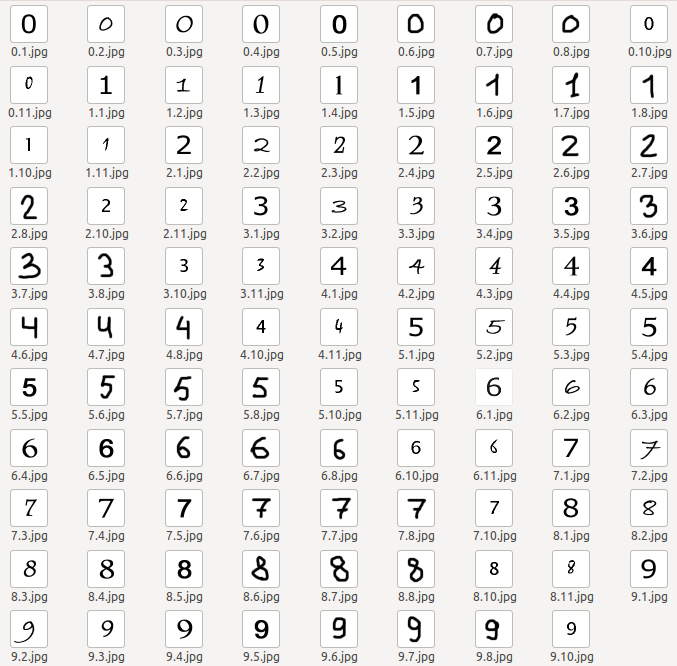
\includegraphics[width=1\linewidth]{vibor.png}}
\caption{Обучающая выборка для нейронной сети.}
\label{ris:vibor}
\end{figure}



\end{document}